\documentclass{standalone}
\usepackage{tikz}
\usepackage{pgfplots}
\pgfplotsset{compat=newest}
\usepackage{mathptmx}
\usetikzlibrary{calc,patterns,decorations.pathmorphing,decorations.markings,matrix,fit,decorations.pathreplacing,arrows.meta,automata,positioning,shapes,chains,spy}
\usetikzlibrary{intersections,through,backgrounds}
\usetikzlibrary{shadows,fadings}
% \usepackage[active,tightpage,pdftex]{preview}
% \PreviewEnvironment{tikzpicture}
\definecolor{dataSampleColor}{HTML}{D23AD0}
\definecolor{discriminatorColor}{HTML}{833EC3}
\definecolor{generatorColor}{HTML}{2B6BD1}
\definecolor{noiseColor}{HTML}{58BD1B}
\definecolor{decisionColor}{HTML}{FED02F}
\begin{document}
  \large
  \centerline{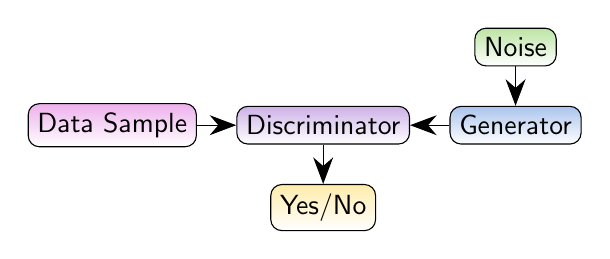
\begin{tikzpicture}[%
    >={Stealth[scale=2.0]},align=center,every node/.style={font=\sffamily}]
    \tikzstyle{state}=[text centered,node distance=0.5cm,%
      rectangle,rounded corners,fill=white,draw=black,%
      minimum width=1.0cm,minimum height=0.45cm]
    % All state styles
    \tikzstyle{dataSample}=[state,top color=dataSampleColor!40]
    \tikzstyle{discriminator}=[state,top color=discriminatorColor!40]
    \tikzstyle{generator}=[state,top color=generatorColor!40]
    \tikzstyle{noise}=[state,top color=noiseColor!40]
    \tikzstyle{decision}=[state,top color=decisionColor!40]
    % All states
    \node (noise) [noise]                                   {Noise};
    \node (generator) [generator,below=of noise]            {Generator};
    \node (discriminator) [discriminator,left=of generator] {Discriminator};
    \node (dataSample) [dataSample,,left=of discriminator]  {Data Sample};
    \node (decision) [decision,below=of discriminator]      {Yes/No};
    % Edges
    \draw [->] (dataSample) -- (discriminator);
    \draw [->] (generator) -- (discriminator);
    \draw [->] (noise) -- (generator);
    \draw [->] (discriminator) -- (decision);
  \end{tikzpicture}}
\end{document}
